\documentclass[letterpaper]{article}
\usepackage{aaai}

\usepackage{times}
\usepackage{helvet}
\usepackage{courier}
\usepackage[T1]{fontenc}
\usepackage[utf8]{inputenc}
\usepackage{graphicx}
\usepackage{url}
\usepackage[bottom,flushmargin]{footmisc}
\renewcommand{\footnotesize}{\tiny}
\setlength{\footnotesep}{0pt}
\setlength{\skip\footins}{4pt}

\frenchspacing
\setlength{\pdfpagewidth}{8.5in}
\setlength{\pdfpageheight}{11in}
\pdfinfo{
/Title (Predicting TCR Cross-Reactivity Before It Reaches a Patient)
/Author (Sergio Mares)
/Keywords (TCR cross-reactivity, pMHC, protein language models, diffusion models, inverse folding, immunotherapy safety)
}
\setcounter{secnumdepth}{2}
\renewcommand{\topfraction}{0.9}
\renewcommand{\bottomfraction}{0.9}
\renewcommand{\textfraction}{0.07}

\begin{document}

\nocopyright
\twocolumn[
\begin{center}
{\large\bfseries Predicting TCR Cross-Reactivity Before It Reaches a Patient\par}
\vspace{2pt}
{\fontsize{8}{9.5}\selectfont Sergio E. Mares, PhD\quad\textperiodcentered\quad Adimab, Mountain View,
CA\quad\textperiodcentered\quad Center for Computational Biology, UC Berkeley\quad
\textperiodcentered\quad Department of Neurosurgery, UCSF\par}
\vspace{6pt}
\end{center}
]

\begin{figure}[t]
\centering
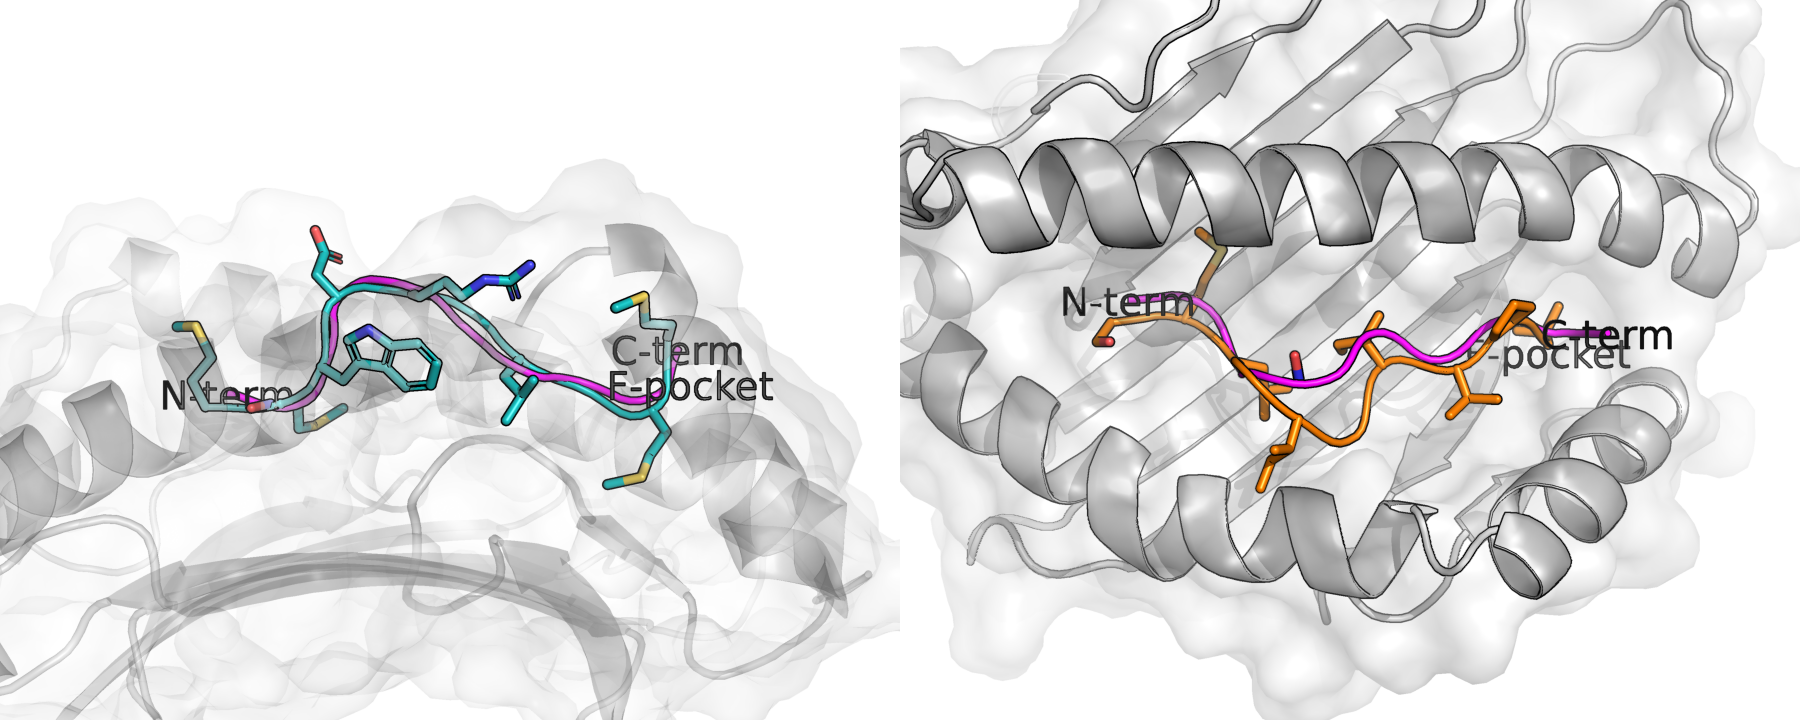
\includegraphics[width=\columnwidth]{../figures/fig2_recovery_crossing/fig2_toprow_proposal.png}
\caption{\textbf{Proposed framework.} A two-state discrimination test in a cross-reactive pMHC--TCR
system. Diffusion models sample from the cognate conformation (teal, left) toward a known off-target
conformation (orange, right), two distinct peptides the same receptor engages. Each generated backbone
(magenta) is scored against both, and credited only if substantially closer to the one it is claimed to
match.}
\label{fig:framework}
\end{figure}

\noindent\textbf{The problem.} Engineered T-cell receptor therapies promise a transformative future for
cancer treatment, and with the 2024 approval of afamitresgene autoleucel that future has begun to
arrive\footnote{N.\ Singh. Approval of the first TCR-based cell therapy. Mol.\ Ther.\ 32:3195, 2024.}.
Cross-reactivity stands between that beginning and routine use. An affinity-enhanced MAGE-A3 receptor
that had cleared extensive preclinical testing killed the first two patients who received it, by
cross-recognizing a self-peptide from the muscle protein titin sharing five of nine residues with the
intended target\footnote{G.\ P.\ Linette et al. Cardiovascular toxicity and titin cross-reactivity of
affinity-enhanced T cells in myeloma and melanoma. Blood 122:863--871, 2013.}. That peptide was
identified only after both deaths\footnote{B.\ J.\ Cameron et al. Identification of a titin-derived
HLA-A1-presented peptide as a cross-reactive target for engineered MAGE-A3-directed T cells. Sci.\
Transl.\ Med.\ 5:197ra103, 2013.}.

\noindent\textbf{Why the field is stuck.} The bottleneck has never been imagination, it has been
throughput. The space of peptides a human cell can present is on the order of $10^{11}$, so exhaustive
experimental testing of one receptor against it is not merely expensive but arithmetically out of reach,
while the aggressive tumors these therapies target leave a clinical window measured in weeks. HLA
polymorphism compounds this. Measured binding data are sparse for most alleles and sparsest for
underrepresented populations, precisely the patients personalized therapy is meant to reach, so the
predictors that might substitute for experiment are weakest where they are needed most. Positional
scanning mutagenesis, the standard alternative, resolves one receptor against one substitution at a time
and does not scale to a space combinatorial in both peptide sequence and receptor identity.

\noindent\textbf{The approach.} The tools to test this at scale have only now come within reach. I would
bring two of my own design. ESMCBA is a binding-affinity predictor built on a protein language model with
domain adaptation, transferring signal from data-rich to data-scarce HLA alleles and extending coverage
into the allelic space conventional predictors abandon\footnote{S.\ Mares, A.\ Espinoza, N.\ M.\
Ioannidis. Continued domain-specific pre-training of protein language models for pMHC-I binding
prediction. PMLR 311:304--325, 2025.}. The second is a structure-guided generative framework in which
diffusion models, conditioned on the geometry of the MHC groove, propose peptides compatible with a given
presentation rather than enumerating them blindly\footnote{S.\ Mares, A.\ Espinoza, N.\ M.\ Ioannidis.
Generation of structure-guided pMHC-I libraries using diffusion models. ICML GenAI and Biology Workshop,
2025.}. Inverse-folding models supply the third component, reading a fixed backbone and decoding which
residues that geometry admits\footnote{H.\ V.\ Ribeiro-Filho et al. Exploring the potential of
structure-based deep learning approaches for T cell receptor design. PLOS Comput.\ Biol., 2024.}, which
localizes the positions a receptor reads. Together they generate a candidate off-target set, rank it, and
localize it (Fig.~\ref{fig:framework}). The instrument is what converts my two tools from proofs of
concept into a working safeguard.

\noindent\textbf{How it is proven.} Each prediction is falsifiable at the bench. The receptor either
engages the flagged peptide or it does not. Validation proceeds in two stages. Retrospectively, the
screen runs blind against receptors whose off-targets are already documented and must recover them. The
MAGE-A3 case is the primary test, since the titin epitope is known and was missed by the methods in use
at the time. A screen that fails to flag it fails outright. Prospectively, top-ranked candidates for a
panel of characterized receptors go to binding measurement and, for those that bind, to functional assay.
This yields a quantity the field currently lacks, a false-negative rate for cross-reactivity prediction
on peptides never seen in training. Both stages apply the same two-state discrimination criterion, so a
candidate counts only when it sits closer to the off-target conformation than to the cognate one, never
on generic proximity to the groove. The validation loop is short enough to close within the appointment,
not left to a successor.

\noindent\textbf{What becomes possible.} A cross-reactivity screen that runs in silico before infusion
turns a lethal surprise into a routine preclinical filter, applied to every candidate receptor rather
than the few that fit an experimental budget, and extended to the allele diversity of real patient
populations rather than the handful with deep binding data. The same framework generalizes past T-cell
receptors to any therapy built on engineered molecular recognition, where the failure mode is likewise
specificity rather than potency. The societal stake is measured in patients, not benchmarks.

\noindent\textbf{Trajectory.} The first problem is chosen because it is winnable inside a year, the
second because it is worth a career. Near term the deliverable is the validated screen and its
false-negative rate. Beyond it lies the harder question the same instrument opens, whether specificity
can be designed at the outset rather than audited afterward, so that receptors are built against the
off-target landscape instead of tested against it.

\noindent Given an instrument of this reach, this is the first thing I would point it at.

\end{document}
